Web Browser haben sich seit der Veröffentlichung von Mosaic, einer der ersten populären Browser, im Jahr 1993 stark weiterentwickelt \cite{EvolutionOfTheWebBrowser}. Das Abrufen und Anzeigen von statischen HTML-Dokumenten wurde mithilfe von JavaScript um interaktive und später um dynamische Inhalte erweitert. Heutzutage können Entwickler komplexe Webanwendungen realisieren \cite{SinglePageApplication}, welche zudem browserunabhängig entwickelt werden können. Durch diese Entwicklung und die vielseitigen Anwendungsfälle, besitzt die Umgebung \enquote{Browser} besondere Eigenschaften, welche nachfolgend beschrieben werden.

\subsection{Browserprodukte}
\label{sec:browserprodukte}

%\begin{wrapfigure}[19]{r}{0.45\textwidth}
%\centering
%\tikzsetnextfilename{cross-browser_metastudie.png}
%\begin{tikzpicture}
%	\begin{axis}[
%		ybar,
%        ymin=0,
%        ymax=350,
%        ytick distance={50},
%		area style,
%		legend style={at={(0.5,-0.10)},anchor=north},
%		nodes near coords,
%		symbolic x coords = {2015, 2016, 2017, 2018, 2019, 2020},
%	]
%		\addplot+[blue,fill opacity=0.2,text opacity=1,ybar,no marks]
%			plot coordinates {
%			(2015,299)
%			(2016,246)
%			(2017,286)
%			(2018,238)
%			(2019,187)
%			(2020,160)
%			};
%		\legend{\strut Suchtreffer bei Google Scholar}
%	\end{axis}
%\end{tikzpicture}
%\caption{Studien zur Browserkompatibilität, eigene Darstellung (vgl. \ref{sec:studien-zur-browser-kompatibilitaet})}
%\label{fig:studien-zur-browser-kompatibilitaet}
%\end{wrapfigure}

\begin{wrapfigure}[19]{r}{0.45\textwidth}
\centering
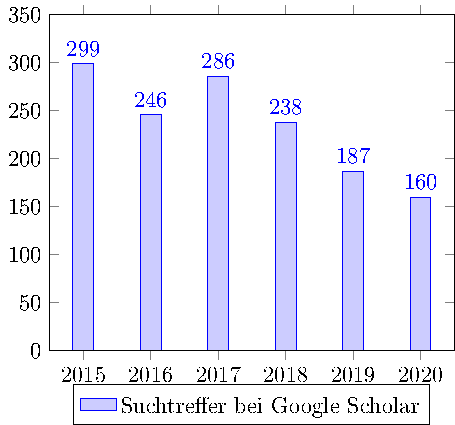
\includegraphics[width=\linewidth]{img/02_theorie/cross-browser_metastudie.png.pdf}
\caption{Studien zur Browserkompatibilität, eigene Darstellung (vgl. \ref{sec:studien-zur-browser-kompatibilitaet})}
\label{fig:studien-zur-browser-kompatibilitaet}
\end{wrapfigure}

Die Vielfalt an Browsern bereitet Webentwicklern immer wieder eine Herausforderung, nämlich ob ein von ihnen bereitgestelltes Produkt für die Nutzer einwandfrei funktioniert, unabhängig der Browserpräferenz des Nutzers. Die Häufigkeit solcher Probleme, auch Cross-Browser-Incompatibilities (XBI) \cite{XBIs} genannt, hat jedoch abgenommen. Dies ist unter anderem durch den Trend von offenen Web-Standards, wie die des W3C \cite{W3CStandards}, erklärbar.

\nomenclature[Fachbegriff]{XBI}{Cross-Browser-Incompatibilities}

Generell lässt sich feststellen, dass auch in der Literatur die Veröffentlichungen in Bezug auf (In-)Kompatibilität von Browsern abnehmen, wie in \autoref{fig:studien-zur-browser-kompatibilitaet} zu betrachten. Dies spricht dafür, dass das Problem von XBIs weniger präsent ist als zuvor. Somit wird die besondere Hürde, die XBIs darstellen, nicht als eine relevante Hürde in dieser Arbeit angesehen.

Im Jahr 2020 gab es weitere Entwicklungen, die die Kompatibilität zwischen Browsern erhöhte. Microsoft ist beim Folgeprodukt zum Internet Explorer, dem Microsoft Edge Browser, von einer proprietären Browser-Engine zu Chromium gewechselt \cite{MicrosoftEdgeChromium} und verwendet denselben Kern wie Chrome und Opera. Ende 2020 wurde zudem der Support für den Internet Explorer 11 eingestellt \cite{MicrosoftInternetExplorerDeprecation}. Im Januar 2021 meldete StatCounter \cite{StatCounterBrowserMarketshare} eine Marktverteilung bei Desktop-Browsern von 65,96\% Chrome, 10,43\% Safari, 8,39\% Firefox, 7,43\% Edge, 2,59\% Opera und 2,54\% Internet Explorer.

\subsection{JavaScript}

Als JavaScript 1997 veröffentlicht und in den NetScape Navigator integriert wurde, gab es die Bedenken, dass das Öffnen einer Webseite dem Betreiber erlaubt Code auf dem System eines Nutzers auszuführen. Damit dies nicht eintritt, wurde der JavaScript Ausführungskontext in eine virtuelle Umgebung integriert, einer sog. Sandbox \cite{LearningJavaScript}.

Die JavaScript-Sandbox bei Browsern schränkt u. A. den Zugriff auf das Dateisystem ein. Auch Zugriff auf native Bibliotheken oder Ausführung von nativem Code ist nicht möglich \cite{TheSpyInTheSandbox}. Browser bieten darüber hinaus aber einige Schnittstellen an, die es erlauben z. B. Daten beim Client zu speichern oder auch Videos abzuspielen.

\nomenclature[Fachbegriff]{CORS}{Cross-Origin Resource Sharing}
\nomenclature[Fachbegriff]{Ajax}{Asynchronous JavaScript and XML}
\nomenclature[Fachbegriff]{W3C}{World Wide Web Consortium}
\nomenclature[Fachbegriff]{XHR}{XMLHttpRequest}

1999 nahm Microsoft im Internet Explorer 5.0 eine neue Methode in ihre JavaScript-Umgebung auf: Ajax (Asynchronous JavaScript and XML) \cite{MDNAjax}. Ajax erlaubt die Datenabfrage von Webservern mittels JavaScript. Hierdurch können Inhalte auf Webseiten dynamisch abgefragt und dargestellt werden, wofür zuvor ein weiterer Seitenaufruf notwendig war. Das Konzept wurde kurz darauf von allen damals gängigen Browsern übernommen. Jedoch fand erst mit der Standardisierung 2006 durch das W3C \cite{TheXMLHttpRequestObject} die Methode bei Entwicklern Anklang und ist seitdem der Grundstein für unser dynamisches und interaktives Web \cite{ResearchOnAJAXTechnology}.

Durch dies wurden Webanwendungen immer beliebter, aber Entwickler klagten darüber, dass Browser die Abfragen von JavaScript nur auf dem bereitstellenden Webserver, also \enquote{same-origin}, erlauben\cite{CrossSiteXHRWithCORS}. Um dies zu ermöglichen, wurde im selben Jahr der Standardisierung von Ajax ein erster Entwurf zur Absicherung von Abrufen domänenfremder Ressourcen eingereicht \cite{AuthorizingCORS}, das sogenannte Cross-Origin Resource Sharing.

Über die Jahre wurde der JavaScript-Standard immer umfangreicher, was Entwicklern erlaubte mächtige Werkzeuge sowie Frameworks zu entwickeln, welche die Erstellung von Webanwendungen vereinfachen. Mit Webanwendungen war es nun möglich, einen großen Teil der Funktionalitäten eines Produktes abzubilden. Diese \enquote{clientbasierten} Anwendungen werden im nächsten Abschnitt näher beleuchtet.

% Im folgenden Abschnitt werden, für diese Arbeit relevante, Sicherheitsvorkehrungen von Browsern vorgestellt und beschrieben - darunter auch Cross-Origin Resource Sharing.

%\subsubsection{Fehleranfälligkeit}
%
%Die Sprache JavaScript stellt an sich auch eine Besonderheit der Umgebung dar. Denn anders als z. B. C, C++, Java gilt sie als fehleranfällig \cite{FastReproducingWebApplicationErrors}. Dies
